\documentclass{article}
\usepackage{style}
\usepackage{ctex}
\usepackage[ruled, linesnumbered, algo2e]{algorithm2e}
\usepackage{amsmath, amsfonts, amsthm}

\usepackage{graphicx, epstopdf}
\usepackage{color}
\usepackage{cite}
\usepackage{indentfirst}
\usepackage{geometry, graphicx}
\usepackage[title]{appendix}
\usepackage{algorithm, algorithmic}
\usepackage{bm}
\usepackage[hidelinks]{hyperref}
\usepackage{multirow}
\usepackage{ulem}
\geometry{left = 5em, right = 5em}
\usepackage{listings}
\usepackage{xcolor}
%% notation macro
\newcommand{\F}{\mathcal F}
\newcommand{\T}{\mathcal T}
\newcommand{\I}{\mathcal I}
\newcommand{\U}{\mathcal U}
\newcommand{\R}{\mathbb R}
\renewcommand{\P}{\mathcal P}
\newcommand{\uP}{ \mathcal \uline P}
\newcommand{\B}{\mathcal B}
%\newcommand{\R}{\mathbb R^2}
\newcommand{\Z}{\mathbb Z}
\newcommand{\C}{\mathbb C}
\newcommand{\laplacian}{\triangle}
\newcommand{\grad}{\nabla}
\renewcommand{\div}{\textrm{div~}}

\newcommand{\diff}[2]{\frac{\partial #1}{\partial #2}}
\newcommand{\difff}[3]{\frac{\parial #1^2}{\partial #2 \partial #3}}
\newcommand{\diFF}[2]{\frac{\partial #1^2}{\partial^2 #2}}
\newcommand{\diam}{\text{ diam }}
%% non-noation macro
\newcommand{\IN}{\text{  in  }}
\newcommand{\ON}{\text{  on  }}
\newcommand{\st}{\text{s.t.  }}
\newcommand{\tbc}{{\color{red}[TBC]}}
\newcommand\ldq\textquotedblleft
\newcommand\rdq\textquotedblright{}
\newcommand\mb\mathbb
\newcommand\mf\mathbf
\newcommand\tf\textbf

\newcommand{\return}{\textbf{return~}}
\DeclareMathOperator{\argmin}{arg~min}
%% enviorment
\newtheorem{proposition}{Proposition}
\newtheorem{definition}{Definition}
\newtheorem{corollary}{Corollary}
\newtheorem{remark}{Remark}


\setlength{\parindent}{1.5em}
\definecolor{mygreen}{rgb}{0,0.6,0}
\definecolor{mygray}{rgb}{0.5,0.5,0.5}
\definecolor{mymauve}{rgb}{0.58,0,0.82}
\lstset{ %
	backgroundcolor=\color{white},      % choose the background color
	basicstyle=\footnotesize\ttfamily,  % size of fonts used for the code
	columns=fullflexible,
	tabsize=4,
	breaklines=true,               % automatic line breaking only at whitespace
	captionpos=b,                  % sets the caption-position to bottom
	commentstyle=\color{green},  % comment style
	escapeinside={\%*}{*)},        % if you want to add LaTeX within your code
	keywordstyle=\color{blue},     % keyword style
	stringstyle=\color{mymauve}\ttfamily,  % string literal style
	frame=single,
	rulesepcolor=\color{red!20!green!20!blue!20},
	% identifierstyle=\color{red},
	language=matlab,
	numbers=left,
}

\makeatletter
\newenvironment{breakablealgorithm}
{% \begin{breakablealgorithm}
		\begin{center}
			\refstepcounter{algorithm}% New algorithm
			\hrule height.8pt depth0pt \kern2pt% \@fs@pre for \@fs@ruled
			\renewcommand{\caption}[2][\relax]{% Make a new \caption
				{\raggedright\textbf{\ALG@name~\thealgorithm} ##2\par}%
				\ifx\relax##1\relax % #1 is \relax
				\addcontentsline{loa}{algorithm}{\protect\numberline{\thealgorithm}##2}%
				\else % #1 is not \relax
				\addcontentsline{loa}{algorithm}{\protect\numberline{\thealgorithm}##1}%
				\fi
				\kern2pt\hrule\kern2pt
			}
		}{% \end{breakablealgorithm}
		\kern2pt\hrule\relax% \@fs@post for \@fs@ruled
	\end{center}
}
\makeatother

%\lhead{\textbf {\showtopic} }
%\chead{} 
%\rhead{\textbf {\showabs} }
%\lfoot{} 
%\cfoot{\thepage}
%\rfoot{} 
%\renewcommand{\headrulewidth}{0.4pt} 
\newtheorem{假设}{假设}

\title{并行与分布式计算}
\date{\today}	
\author{
	敖睿成 1900012179\\
	数学科学学院\\
	\texttt{archer\_arc@pku.edu.cn} \\
}
\begin{document}

	\maketitle
	\thispagestyle{fancy}
	\tableofcontents
	\section{摘要}
	本次任务要求我们使用 MPI 的 Send/Recv 原语实现 In-place的Allreduce算子。我们利用上课时所教授及实例代码,同时查阅资料和文献\cite{cai2021synthesizing,gibiansky2017bringing,sergeev2018horovod,allreduce},实现了五种算法:Star-Allreduce, Circle-Allreduce, Recursive-Allreduce,  Butterfly-Allreduce 以及 Ring-Allreduce。对每一种算法,报告中都给出了相应的理论分析和在不同数据大小下的数值实验结果。此外,我们也将其与 MPI 所提供的 Allreduce 进行了比较,讨论并分析了不同算法的表现差异及优劣。
	
	\section{算法描述及分析}
		
	根据 \cite{allreduce}, 我们对通信过程作出以下假设
	\begin{假设}
		在通信过程中,任两个进程的点对点通信不受到其它进程的通信干扰。带宽假设每个进程发送单位数据所需要的时间为$t$,单位数据的运算时间为$c$。每次通信额外的固定时间为$\alpha$。数据大小为$Size$,进程数为$Commsize$.
	\end{假设}
为了实现节省空间的In-place Allreduce, 我们均需要对数据进行切片,假设每次切片数为$N$。  
\subsection{Star-Allreduce}
Star-Allreduce 顾名思义,其拓扑结构为星状,由一个进程 0 连接其它所有进程。通信时,其它进程同时向进程 0 发送数据,在进程 0 进行计算后重新发给其它所有进程,是 Reduce/Broadcast 的模式。
\begin{figure}[H]
			\centering
	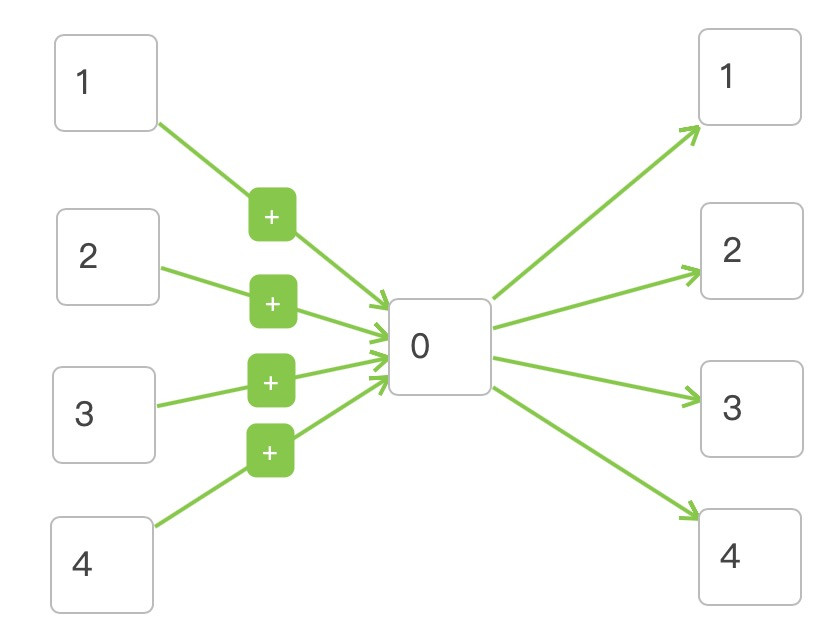
\includegraphics[width=0.6\linewidth]{./fig/star}
	\caption{$Commsize = 5$时的 Star-Allreduce 图例\label{fig:star}}
\end{figure}
其总共通信了$2N*Commsize$轮,总体的通信耗时约为 $2N(\alpha+t*Size/N)*Commsize+(Commsize-1)*Size*c$ (注意到其中一个叶进程向根进程发送的时候其它的进程都在等待)。其缺点是明显的,每次将所有的数据同时发送到同一个进程,又从同一个进程发出,可能会面临严重的带宽瓶颈问题。

\subsection{Circle-Allreduce}
Circle-Allreduce 和上课时所讲的击鼓传花是一样的,共分为两个部分进行。第一部分$0\rightarrow1\rightarrow2\cdots\rightarrow Commsize-1$,每次传递数据并求和。第二部分$Commsize-1\rightarrow Commsize-2\rightarrow\cdots\rightarrow1$。这样的总通信耗时约为 $2N(\alpha+t*Size/N)*(Commsize-1)+(Commsize-1)*Size*c$。它相比 Star-Allreduce 唯一的优势在于可以避免所有的通信集中在同一个进程带来的带宽问题,但其异步通信也增加了通信的轮数,从而增大时间开销。
\begin{figure}[H]
	\centering
	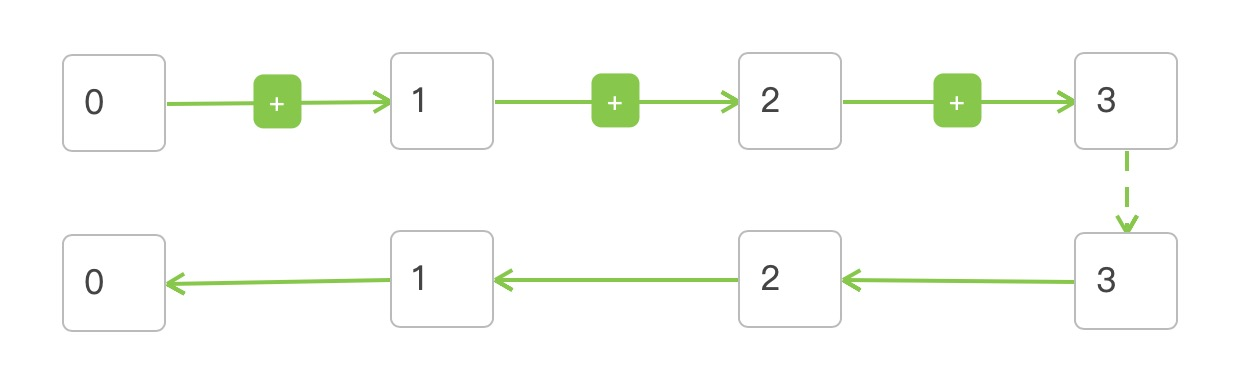
\includegraphics[width=0.6\linewidth]{./fig/circle}
\caption{$Commsize = 4$时的 Circle-Allreduce 图例,虚线表示没有实际的通信\label{fig:circle}}
\end{figure}

\subsection{Recursive-Allreduce}
Recursive-Allreduce 是一种使用二叉树结构进行归并的 Allreduce 算法,其算法可以描述如下
\begin{algorithm}[H]
	\caption{Recursive-Allreduce}
	\begin{algorithmic}[1]
			\STATE{$\beta_0 = \min_{\beta}\{2^\beta \ge Commsize\}.$}
			\FOR{$k= \beta_0 :-1 : 0 $}
			\IF{$rank >= 2^k$}
			\STATE{	Process $rank$ send data to Process $rank-2^{k}$}
			\ELSIF{$rank+2^{k}<Commsize$}
			\STATE{ Process $rank$ receive data from Process $rank+2^{k}$ and compute the sum}
			\ENDIF
			\ENDFOR
			\FOR{$k=0:\beta_0-1$}
			\IF{$rank >= 2^k$ and $rank < Commsize$}
			\STATE{ Process $rank$ receive data from Process $rank-2^{k}$}
			\ELSIF{$rank +2^k < Commsize$}
			\STATE{ Process $rank$ send data to Process $rank+2^k$}
			\ENDIF
			\ENDFOR 
	\end{algorithmic}
\end{algorithm}
	相当于由进程 $0$生成的一个二叉树(其叶子进程可能不满),第$k$层由进程$0,1,\dots,2^k-1$构成。第一部分由每个叶子向父亲发送数据并求和(实际上其中一个叶子和父亲是一样的),第二部分由每个进程向自己的叶子(如果存在)发送数据(广播阶段)。其时间复杂度约为 $2N*(log_2Commsize)*(\alpha+t*Size/N)+(\log_2 Commsize)*Size*c$. 可以看到其本身不依赖于$Commsize$是否为$2$的幂次,不但解决了带宽问题,也显著减少了通信所需要的轮数,是比 Circle-Allreduce 和 Star-Allreduce 都高效的算法。
	\begin{figure}[H]
		\centering
		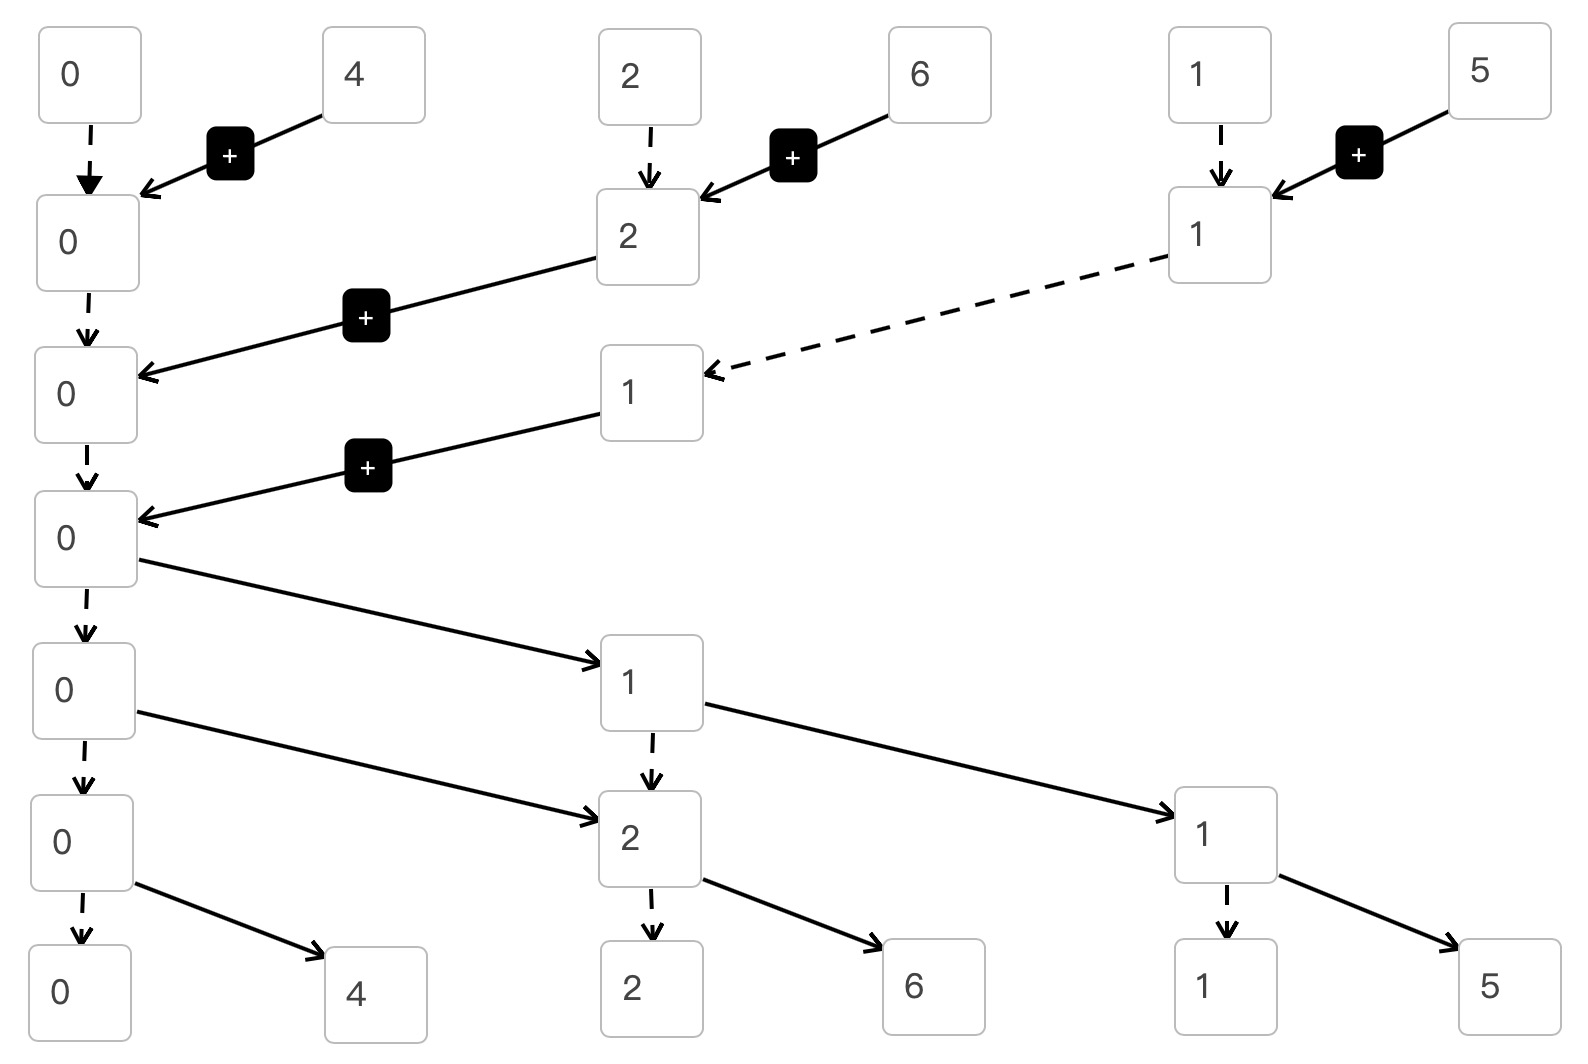
\includegraphics[width=0.6\linewidth]{./fig/recursive}
		\caption{$Commsize = 6$时的 Recursive-Allreduce 图例,虚线表示没有实际的通信\label{fig:recursive}}
	\end{figure}
\subsection{Butterfly-Allreduce}
Butterfly-Allreduce 同样是基于归并的想法。注意到在 Recursive-Allreduce 算法当中,越是靠近“中段”的通信轮次,其空闲的进程也就越多,基于充分利用的思想,Butterfly 算法每次采取“交换数据”的方法,而非单向的发送,每一次交换的进程就被划为了“同组”,这样同一组的进程保管着相同的数据,可以尽可能多地在每一轮利用进程,减少了通信所需要的轮次。算法的描述如下
\begin{breakablealgorithm}
	\caption{Butterfly-Allreduce}
	\begin{algorithmic}[1]
			\STATE{$\beta_0 = \min_{\beta}\{2^\beta \ge Commsize\}.$}
			\FOR{$k=0:\beta_0-1$}
			\STATE{$stepsize=2^k$}
			\IF{$rank \mod stepsize < stepsize/2$}
			\STATE{$dest=rank+stepsize/2$}
			\ELSE
			\STATE{$dest=rank-stepsize/2$}
			\ENDIF
			\IF{$dest<Commisze$}
			\STATE{ Exchange data between Process $dest$ and $rank$, then compute the sum}
			\ELSIF{$stepsize>2$}
			\STATE{$dest = rank - rank\mod stepsize$}
			\IF {$dest != rank$}
			\STATE{ Process $rank$ receive data from Process $dest$}
			\ENDIF
			\ENDIF
			\IF{$rank \mod stepsize == 0$ and $rank + stepsize > Commsize$}
			\FOR{$not\_matched\_count = 1 : rank+stepsize-Commsize$}
			\STATE{$dest=rank+stepsize/2-not\_matched\_count$}
			\STATE{ Process $rank$ send data to Process $dest$}
			\ENDFOR
			\ENDIF
			\ENDFOR
	\end{algorithmic}
\end{breakablealgorithm}

其可以描述为,我们最初有$Commsize$个组,每次将相差 $stepsize$ 的进程进行两两配对,交换同一对进程的数据并求和,这样相邻连续的 $2*stepsize$ 个进程的数据都是相同的,它们被划为同一组,最终可以将所有的进程并为同一组。当然,当 $Commsize$ 不为 $2$ 的幂次的时候每次可能会出现落单进程,易于证明这样的情况只会发生在最右边,那么我们可以将同一组最左边的进程上的数据分发给这一组余下的进程。这样经过$[log_2 Commsize]$轮后就完成了 $Allreduce$,其通讯总耗时约为  $N(\log_2Commsize)*(\alpha+t*Size/N)+(\log_2 Commsize)*Size*c$。

此外,上面的计算量也是能够减半的,原因在于,我们上面的算法当中将配对的进程同时发送、接收并分别求和,实际上可以先各自将一半的数据分别发送/接收,分别求和后再进行一半数据的发送/接收。这样通讯总耗时约为 $2N(\log_2Commsize)*(\alpha+t*Size/(2N))+(\log_2 Commsize)*Size/2*c$,尽管通讯的固定时长增加了,但却减少了一半的计算量。
	\begin{figure}[H]
	\centering
	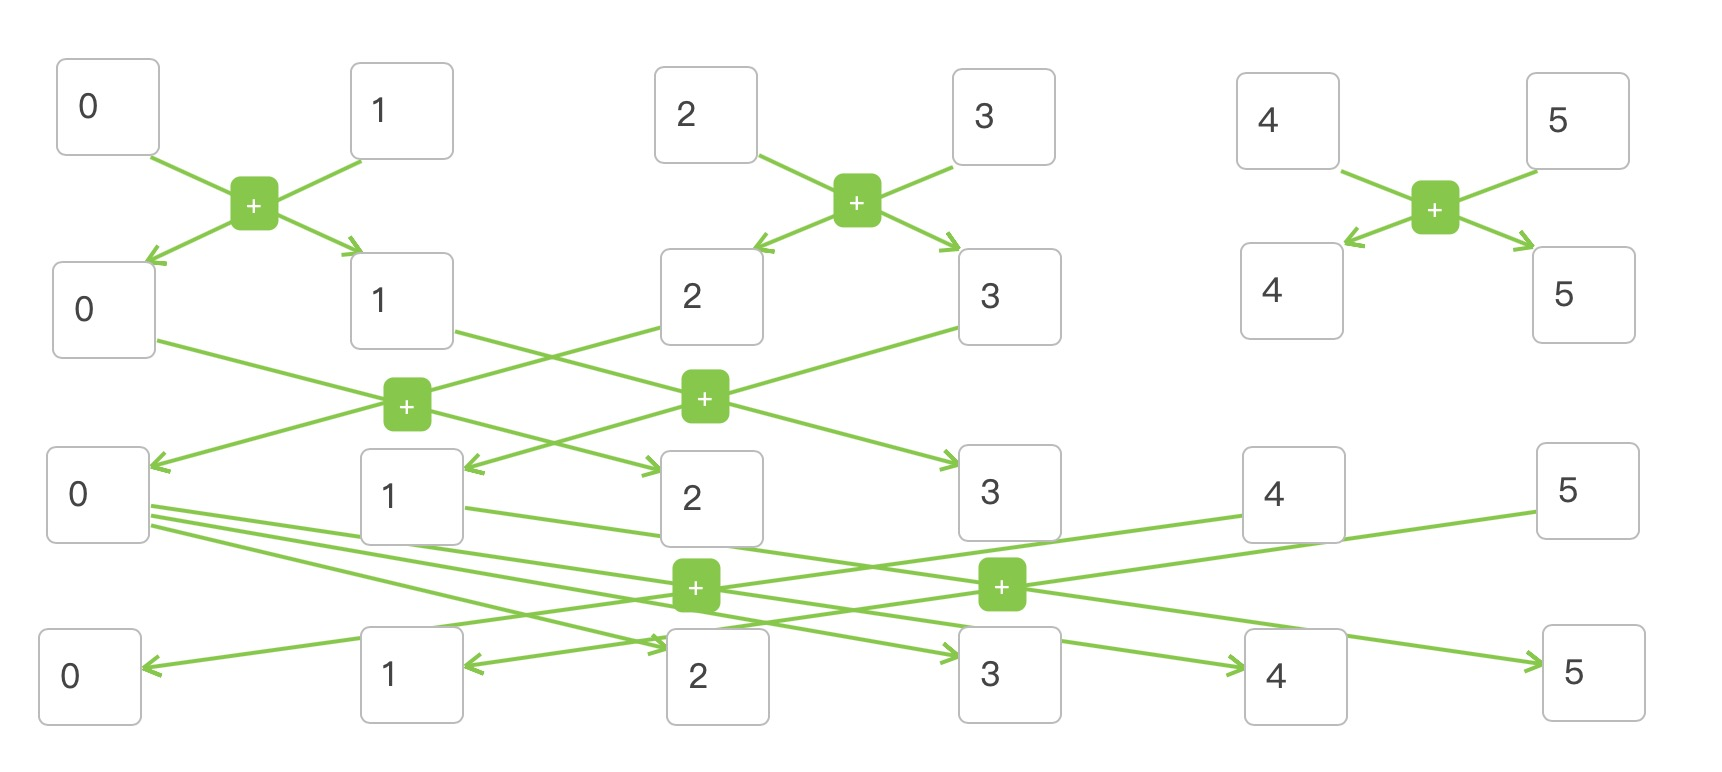
\includegraphics[width=0.8\linewidth]{./fig/butterfly}
	\caption{$Commsize = 6$时的 Butterfly-Allreduce 图例\label{fig:butterfly}}
\end{figure}

\subsection{Ring-Allreduce}
Ring-Allreduce 可以看作是 Circle-Allreduce 的改进,其特点在于利用了 Circle-Allreduce 当中每轮通信闲置的进程,先将数据切片成 $Commsize$ 份,通信共分成两部分进行。第一部分在第 $k$ 轮将进程 $i$ 的第 $i-k+1$ 段数据发送给进程 $i+1$ (按mod $Commsize$来算),共进行 $Commsize-1$ 轮。第二部分在第 $k$ 轮将进程 $i$ 的第 $i-k+2$ 段数据发送给进程 $i+1$。这样共 $2Commsize-2$轮后,就完成了 Allreduce,其示意图如下
	\begin{figure}[H]
\centering
	\begin{minipage}{0.48\linewidth}
		\centering
	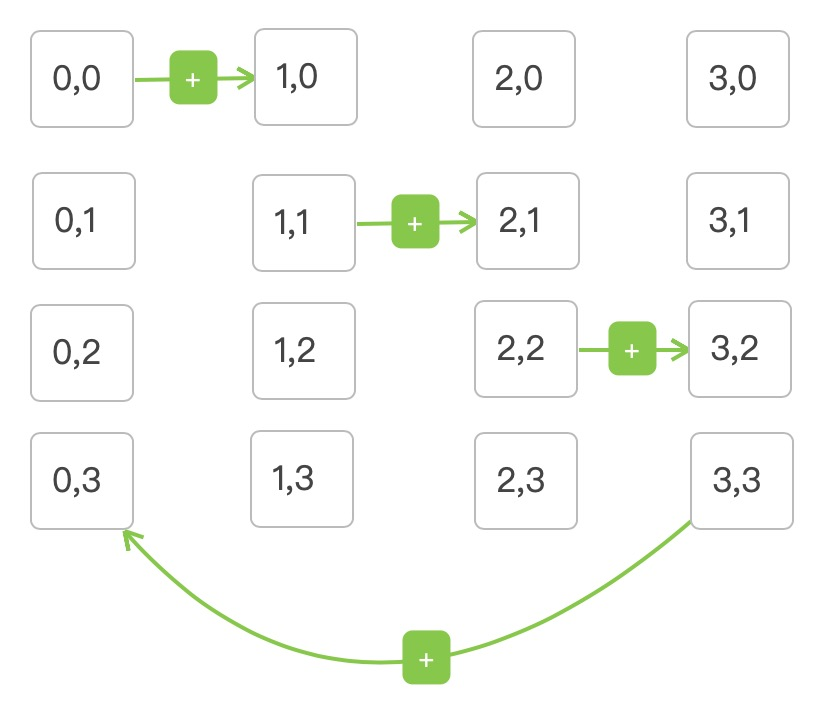
\includegraphics[width=0.8\linewidth]{./fig/ring1}
	\\第一部分
	\end{minipage}
			\begin{minipage}{0.48\linewidth}
				\centering
			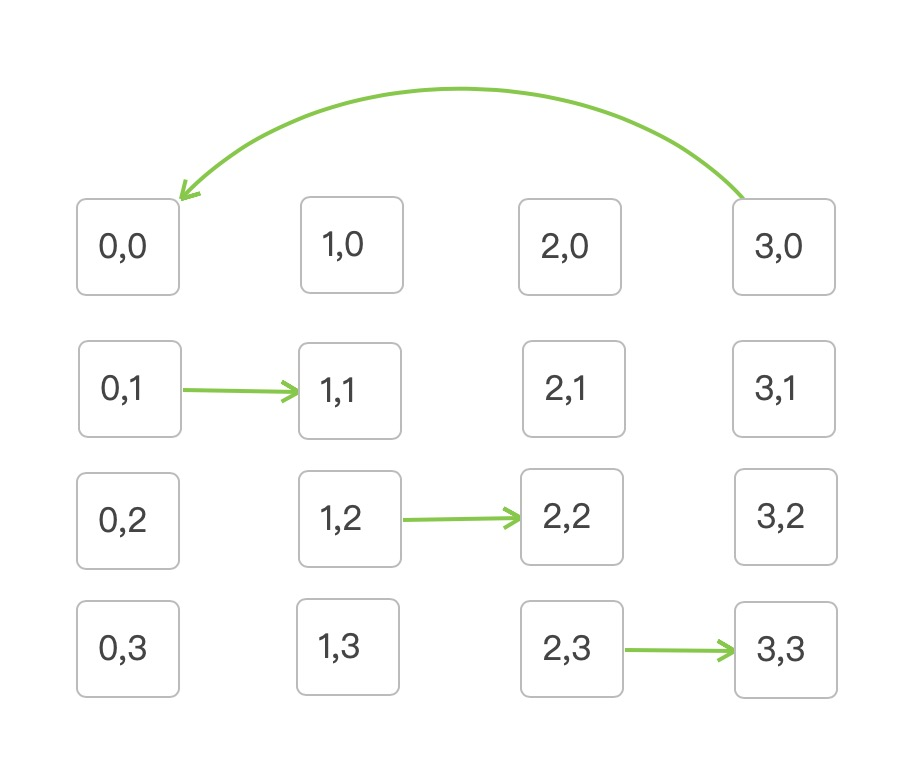
\includegraphics[width=0.8\linewidth]{./fig/ring2}
			\\第二部分
			\end{minipage}
	\caption{$Commsize = 4$时的 Ring-Allreduce 图例\label{fig:ring}}
\end{figure}
可以计算得耗时约为$2*(Commsize-1)*(\alpha+t*Size/Commsize)+\frac{Commsize-1}{Commsize}*Size*c$。可以看出,其耗时在我们报告里的假设下,是所有算法当中最优的。这得益于它有效地减少了计算所耗的时间,同时也有效地减少了带宽,我们不需要很大的缓冲区,并且所有的进程都同时参与了每一轮通信。
\subsection{总结}
上面的每种 Allreduce 算法的时间和空间缓存开销可以总结为下表
\begin{table}[H]
	\centering
	\begin{tabular}{c|cc}
		算法 & 时间开销 & 缓存开销 \\ \hline 
		Star-Allreduce &$ 2N(\alpha+t*Size/N)(Commsize-1)+(Commsize-1)*Size*c$ &$\mathcal O(Size/N) $ \\
		Circle-Allreduce &$2N(\alpha+t*Size/N)(Commsize-1)+(Commsize-1)*Size*c$ &$\mathcal O(Size/N)$ \\
		Recursive-Allreduce & $2N(log_2Commsize)(\alpha+t*Size/N)+(\log_2 Commsize)*Size*c$ & $\mathcal O(Size/N)$\\
		Butterfly-Allreduce &$2N(\log_2Commsize)(\alpha+t*Size/(2N))+(\log_2 Commsize)*Size*c$&$\mathcal O(Size/N)$\\
		Ring-Allreduce &$2(Commsize-1)(\alpha+t*Size/Commsize)+\frac{Commsize-1}{Commsize}*Size*c$&
		$\mathcal O(Size/Commsize)$
	\end{tabular}
\caption{不同算法的性能比较}
\end{table}
从表中可以看到,越往下面的算法性能就越好。前两种算法基本上就是直接 Reduce/Broadcast 或稍微改编,基本每次通信时其它的进程都空闲着,并没有做到并行。而 Recursive-Allreduce 通过同时发送/接收的二叉树结构,将通信的轮数降到了 $log_2 Commsize$ 级别,但是仍然有很多的闲置进程。Butterfly-Allreduce 则将 Recursive-Allreduce 进行了进一步的改进,但问题在于有 $log_2 Commsize-1$ 倍的计算都是重复的。最后的 Ring-Allreduce 可以充分利用带宽,同时也没有重复计算,做到了每个进程都在计算不同的数据。因此,当 $Commsize$ 和数据大小 $Size$ 较小时,这几种方法没有明显的差别,当数据越来越大时,Star-Allreduce 就可能出现带宽瓶颈,当进程数也很大时,Ring-Allreduce 就明显地优于其它的算法。此外,上面的 Ring-Allreduce 将数据切分成了 $Commsize$ 份,当数据过大时,可能需要切成更多份,分段进行 Ring-Allreduce。
\section{数值结果及分析}
我们分别对 $Size = 1024^2, 4*1024^2, 8*1024^2, Commsize=4,5,\dots,16,N = Commsize,$ $Commsize*4,Commsize*5$都进行了数值实验。并且我们都进行了对应算法的 Out-place 版本便于比较。为了排除服务器造成的不稳定性,数值结果是当$Size=1024^2, 4*1024^2$时对$100$次实验取平均值,$Size=8*1024^2$时对$30$次实验取平均值(尽管如此,我们的结果依然会出现很多不确定因素,可能一次 baseline 的实验就会超过10分钟)。出于篇幅考虑,我们仅在下面列出部分结果,其余的结果可以在 ../code/result 目录下找到。其中误差为$100$次实验单次最大误差的平均值,前面加了O的表示 Out-place 版本的算法。相关的代码和结果可以在../Code文件夹找到,README.txt中有详细的解释。
\begin{table}[H]
	\centering
	\begin{tabular}{c|cc|cc|cc}
		 & \multicolumn{2}{|c|}{$Datasize=1024^2$}  &\multicolumn{2}{|c|}{$Datasize=4*1024^2$}&\multicolumn{2}{c}{$Datasize=8*1024^2$}\\\hline
		算法 &时间 &误差 &时间 &误差 &时间 &误差\\ \hline
		Baseline &0.0049&-&0.028&-&0.46&-\\
		Star& 0.0070&2.38e-07&0.038&2.38e-07&0.068& 2.38e-07\\ 
		Circle &0.0051&2.38e-07&0.029&2.38e-07&0.074&2.38e-07\\ 
		Recursive &0.0043&0&0.021&2.38e-07&0.051&2.38e-07 \\
		Butterfly &0.0036&2.38e-07&0.018&2.38e-07&0.048&2.38e-07\\
		Ring &0.0036&4.76e-07&0.017&4.76e-07&0.030&4.76e-07\\
		Ostar &0.0062&2.38e-07&0.032&2.38e-07&0.79&2.38e-07\\
		Ocircle &0.0068&2.38e-07&0.030&2.38e-07&0.43&2.38e-07\\
		Orecursive &0.0041&0&0.022&0&0.51&0\\
		Obutterfly &0.0038&2.38e-07&0.022&2.38e-07&0.26&2.38e-07
	\end{tabular}
\caption{$Commsize = 4, N = Commsize*4$时的结果}
\end{table}
\begin{table}[H]
	\centering
	\begin{tabular}{c|cc|cc|cc}
		& \multicolumn{2}{|c|}{$Datasize=1024^2$}  &\multicolumn{2}{|c|}{$Datasize=4*1024^2$}&\multicolumn{2}{c}{$Datasize=8*1024^2$}\\\hline
		算法 &时间 &误差 &时间 &误差 &时间 &误差\\ \hline
		Baseline &0.0082&- &0.052&- &0.45&-\\
		Star& 0.0093&4.76e-07&0.068&4.76e-07&0.34&4.76e-07\\
		Circle &0.0066&4.76e-07&0.050&4.76e-07&0.11&4.76e-07\\
		Recursive &0.0062&4.76e-07&0.041&4.76e-07&0.19&4.76e-07\\
		Butterfly &0.0084&4.76e-07&0.042&4.76e-07&0.16&4.76e-07\\
		Ring &0.0042&4.76e-07&0.034&9.53e-07&0.25&9.53e-07\\
		Ostar &0.0080&4.76e-07&0.047&4.76e-07&0.56&4.76e-07\\
		Ocircle &0.0094&4.76e-07&0.041&4.76e-07&0.79&4.76e-07\\
		Orecursive &0.0062&4.76e-07&0.035&4.76e-07&0.32&4.76e-07\\
		Obutterfly &0.0082&4.76e-07&0.047&4.76e-07&0.30&4.76e-07
	\end{tabular}
	\caption{$Commsize = 5, N = Commsize*4$时的结果}
\end{table}
\begin{table}[H]
	\centering
	\begin{tabular}{c|cc|cc|cc}
		& \multicolumn{2}{|c|}{$Datasize=1024^2$}  &\multicolumn{2}{|c|}{$Datasize=4*1024^2$}&\multicolumn{2}{c}{$Datasize=8*1024^2$}\\\hline
		算法 &时间 &误差 &时间 &误差 &时间 &误差\\ \hline
		Baseline &0.011&-&0.47&-&140.47&-\\
		Star& 0.032&2.86e-06&0.44&2.86e-06&25.33&2.86e-06\\
		Circle &0.021&2.86e-06&0.43&2.86e-06&28.88&2.86e-06\\
		Recursive &0.0078&1.91e-06&0.096&1.91e-06&16.72&1.91e-06\\
		Butterfly &0.010&1.91e-06&0.07&1.91e-06&16.10&1.91e-06\\
		Ring &0.013&2.86e-06&0.10&2.86e-06&19.40&3.81e-06\\
		Ostar &0.028&2.86e-06&0.13&2.86e-06&16.34&2.86e-06\\
		Ocircle &0.033&2.86e-06&0.69&2.86e-06&66.39&2.86e-06\\
		Orecursive &0.0088&1.91e-06&0.062&1.91e-06&40.30&1.91e-06\\
		Obutterfly &0.026&1.91e-06&0.17&1.91e-06&90.72&1.91e-06
	\end{tabular}
	\caption{$Commsize = 16, N = Commsize*4$时的结果}
\end{table}
从结果整体来看,与我们的分析是较符合的,并且我们的成功性不依赖于进程数和数据大小的倍数和整除关系,但由于服务器的不稳定性,导致可能有时会出现一些极端的情况(例如baseline有过一次跑了10分钟),这是我们即使取平均也难以消除的。因此,也会出现在我们分析当中性能较好的算法在某次实验当中反而不如分析中性能较差的算法,但这样的结果毕竟是少数,从而也可以说明我们的拓扑结构和分析的合理性。Out-place 的算法需要开辟等同于数据大小的空间,在$Datasize$较小时,可以看出和 In-place 的算法差距不大甚至可能更快,但当数据量很大的时候,In-place 算法的优势就体现了出来,可以看到,我们表格中当$Datasize=8*1024^2$时,In-place 算法的效果显著好于 Out-place 的,基于同样的理由,我们也可以合理推测,由于 Ring-Allreduce 中选取固定的切片长 $Commsize$,而其它的选取切片长 $Commsize*4$,当进程数增加时,其它 In-place 算法也会表现出更好的性质,这一点也在数值结果中有体现。

另一方面,我们也对结果的误差进行分析,我们观察到在某些时候相同的算法在不同的进程数下的实验出现了不同的误差,也会有不同的算法在同一实验中出现了相同的误差,这是由于加法的顺序不同对舍入误差造成的影响。值得注意的一点是,观察到$Commsize=4$时 Recursive-Allreduce的误差为0,可以推测此时我们的求和顺序和标准库函数是相同的。假设 $\mathbf{u}$是 float 的机器精度,易于得到 Recursive-Allreduce, Butterfly-Allreduce 的理论舍入误差上界为 $\mathcal O(\mathbf u\log_2Commsize)$,而另外三种算法的理论舍入误差上界为 $\mathcal O(Commsize*\mathbf u)$。通过对比我们表中的实验结果不难看出确实是符合的。

	\bibliographystyle{unsrt}  
	\nocite{*}
\bibliography{ref}
\end{document}